\section{Experiments}

\subsection{Experimental Setup}
\label{sec:setup}

\paragraph{Tasks and inputs.}
Our main collection contains 50 PyTorch-to-MindSpore migration tasks covering tensor operations, CNNs, image MLPs, Transformer components, small language models, and parameter and optimizer interfaces. Twelve task entries reuse existing native source programs; the other entries use programs authored from public interfaces and declared semantics. The 50 task identifiers correspond to 29 distinct source-and-contract pairs drawn from 24 source files. Conditions with identical source, contract, initial candidate, method, and evaluation inputs are executed once and associated with their corresponding identifiers. Main-table acceptance uses the 50 identifiers, while token totals count actual calls over the 29 distinct pairs. The cross-language collection contains 18 complete Java/DJL sources, including application programs and textbook examples, translated to Python/PyTorch. Its completed initial translations are shared by the repair methods.

\paragraph{Verification.}
Every method in a collection receives the same source programs and public contracts and is evaluated with the same inputs, initial states, seeds, and thresholds. The main collection uses seeds 101, 202, and 303. Operator tasks compare forward values and applicable input gradients; model tasks add parameter gradients; tasks with a training entry point add two consecutive training steps and parameter updates. Parameter and optimizer tasks check their declared enumeration, gradient assignment, or update behavior. Shapes, data types, initial values, and trainability must match. Absolute/relative tolerances are $10^{-4}/10^{-4}$ for forward values, $10^{-4}/10^{-3}$ for gradients, and $10^{-5}/10^{-3}$ for updates; BF16 matrix multiplication uses absolute tolerance $10^{-2}$. Acceptance requires all applicable checks on all three seeds and observed target-backend execution. Cross-language acceptance compares two consecutive training steps after preprocessing, with seed 101 for visible tests and 202 and 303 for confirmation. Public inputs comprise the source, contract, current candidate, and test observations; reference measurements and healthy target implementations remain in the evaluation process.

\paragraph{Methods and budgets.}
The MindSpore comparison includes LaDiM, SWE-agent~\citep{yang2024sweagent}, MatchFixAgent~\citep{ibrahimzada2025matchfixagent}, Direct LLM, CodeTransEngine's direct translation configuration~\citep{macedo2025codetransengine}, and MSAdapter~\citep{openi2025msadapter}. The three repair agents start from the same Direct LLM translation. SWE-agent uses its native tools and controller; MatchFixAgent retains its analysis and repair orchestration through a shared DeepSeek tool backend. CodeTransEngine generates its own translation through the native direct path, and MSAdapter uses its native interface mapping. The cross-language comparison includes the three agents, a whole-file test-guided repair loop, Direct LLM, and InterTrans's search over direct and intermediate-language paths. Native method prompts, parsers, and retry policies are retained. All model calls use the configured DeepSeek backend. Repair agents have a shared limit of 40 calls, 120,000 output tokens, 1,800 seconds, and four external submissions per task; LaDiM allows eight calls per investigation or repair stage. Each agent call allows up to 16,384 output tokens. Initial translation and whole-file repair allow up to 131,072 output tokens per call, with four repair rounds for the latter. Submission checkpoints record the current candidate after the native method's internal actions.

\paragraph{Cost and acceptance.}
We report end-to-end prompt plus completion tokens, including the shared initial translation and all subsequent diagnosis, repair, and failed calls. Shared translations are attributed once within each method's total. Provider-reported cached input tokens remain part of token use. Functional failures and incomplete runs remain in the declared denominator and cost totals, including InterTrans's incomplete generation calls. Acceptance counts score the current candidate at the stated checkpoint. Additional component, signal, and framework protocols appear in Appendix~\ref{sec:supplementary-protocols}.

\subsection{Main Experiments}
\label{sec:main-results}

\begin{table}[t]
\caption{Migration acceptance and end-to-end model use. Each panel compares methods on a common collection and acceptance protocol: 50 PyTorch-to-MindSpore tasks in (a), and 18 Java/DJL-to-Python/PyTorch tasks in (b).}
\label{tab:main-results}
\centering
\small
\setlength{\tabcolsep}{5pt}
\begin{tabular*}{\linewidth}{@{\extracolsep{\fill}}lrrr@{}}
\toprule
\textbf{Method} & \textbf{Accepted} & \thead{Total tokens\\(millions)} & \thead{Model\\calls} \\
\midrule
\multicolumn{4}{l}{\textit{(a) PyTorch to MindSpore}} \\
Direct LLM & 29/50 & 0.429 & 29 \\
CodeTransEngine (direct)~\citep{macedo2025codetransengine} & 31/50 & 0.280 & 29 \\
MSAdapter~\citep{openi2025msadapter} & 15/50 & 0.000 & 0 \\
SWE-agent~\citep{yang2024sweagent} & 44/50 & 20.831 & 1,097 \\
MatchFixAgent~\citep{ibrahimzada2025matchfixagent} & 50/50 & 12.097 & 619 \\
\textbf{LaDiM (ours)} & \textbf{50/50} & 5.159 & 326 \\
\midrule
\multicolumn{4}{l}{\textit{(b) Java/DJL to Python/PyTorch}} \\
Direct LLM & 1/18 & 0.694 & 18 \\
InterTrans~\citep{macedo2024intertrans} & 1/18 & 2.286 & 89 \\
Test-guided repair & 7/18 & 4.475 & 71 \\
SWE-agent~\citep{yang2024sweagent} & 8/18 & 24.321 & 682 \\
MatchFixAgent~\citep{ibrahimzada2025matchfixagent} & 8/18 & 28.355 & 524 \\
\textbf{LaDiM (ours)} & 9/18 & 21.479 & 345 \\
\bottomrule
\end{tabular*}

\end{table}

LaDiM achieves 50/50 acceptance on the unified MindSpore collection, matching MatchFixAgent while using 57.4\% fewer tokens (Table~\ref{tab:main-results}a). Their common initial translation passes 29/50 task identifiers. Both methods repair the remaining 21 and preserve all initially accepted programs. Direct LLM and CodeTransEngine provide inexpensive initial translations, while the verification and repair loop extends acceptance to the complete collection. This gain shows the value of investigating the discrepancies left by a translation before accepting its training behavior.

The comparison also connects coverage with the amount of interaction required to obtain it. LaDiM uses 326 end-to-end model calls, compared with 619 for MatchFixAgent, at the same final acceptance. SWE-agent accepts 44/50 with 1,097 calls. LaDiM's investigation records the observed discrepancies and candidate locations before repair; subsequent calls can use this evidence to test and revise a concrete hypothesis. Section~\ref{sec:fault-characterization} examines how this workflow behaves on initially correct and initially faulty inputs.

\subsection{Analysis Experiments}
\label{sec:fault-characterization}

\paragraph{Repair effectiveness and efficiency.}
LaDiM's token advantage is distributed across the collection: it uses fewer tokens than MatchFixAgent on 27 of the 29 distinct input pairs (Figure~\ref{fig:repair-comparison}b). These include eight of the nine initially faulty pairs and 19 of the 20 initially accepted pairs. On the faulty pairs alone, its additional investigation and repair use 3.32 million tokens, compared with 6.53 million for MatchFixAgent, a reduction of 49.2\%. The advantage therefore extends to the tasks that require corrective edits. On initially accepted inputs, LaDiM finishes after investigation and confirmation, preserving the candidate; the corresponding additional use is 1.41 million tokens, compared with 5.14 million for MatchFixAgent. Both accurate repair and completion of already-correct tasks contribute to end-to-end efficiency.

\begin{figure}[t]
\centering
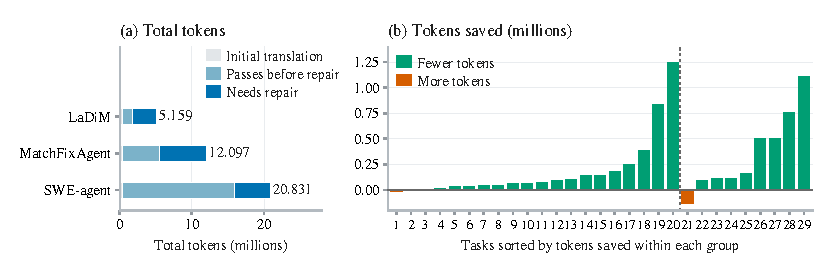
\includegraphics[width=\linewidth]{figures/repair_comparison.pdf}
\caption{Token use on the common MindSpore collection. (a) End-to-end totals for the three repair agents. (b) Each point compares LaDiM and MatchFixAgent on one of the 29 distinct source-and-contract pairs, with symbols indicating the initial translation's acceptance. Both methods accept every pair. Points below the dashed line indicate lower token use by LaDiM. Both axes use logarithmic scales.}
\label{fig:repair-comparison}
\end{figure}

\paragraph{Budgeted repair.}
LaDiM reaches 46/50 acceptance after one repair submission and 50/50 after two, retaining full acceptance at the four-submission budget. Among the nine distinct failing initial translations, seven are repaired after the first submission and two after the second. Returning the remaining measured discrepancies thus resolves cases that the first edit leaves incomplete. MatchFixAgent reaches 50/50 within its first external submission through its internal analysis and repair orchestration. Its larger call and token totals show why external submissions and internal model interactions describe different aspects of repair effort.

\paragraph{Training signals and detection latency.}
The diagnostic study follows four models over 50 steps and three seeds. Under per-step synchronization, each target model starts the checked step from the source state, allowing a discrepancy to be associated with the current computation. Correct translations pass the recorded checks, with a maximum loss difference of $3.815\times10^{-6}$. The fault trajectories show complementary signals: a gradient error can preserve loss agreement, and an update error can preserve both the forward computation and the current gradient.

When the target retains its own state, these errors influence later forward computations. In Figure~\ref{fig:gradient-drift}, gradient and update checks detect their respective faults at step~1 in all 12 runs per panel. The mean loss difference crosses its threshold at steps 31 and 18, while individual loss trajectories cross within the observation window in 3/12 and 4/12 runs. The direct signals therefore supply actionable evidence before loss drift becomes a dependable indicator. This timing explains why the repair process checks the computations that produce a training update.

\subsubsection{Generalization Across Languages}
LaDiM accepts 9/18 Java/DJL-to-Python/PyTorch translations, compared with 8/18 for both SWE-agent and MatchFixAgent and 7/18 for test-guided repair (Table~\ref{tab:main-results}b). The shared initial translations contain one accepted program, which all four repair methods preserve. LaDiM repairs eight additional tasks. It accepts all eight tasks accepted by MatchFixAgent and additionally repairs the concise recurrent-network example. Relative to SWE-agent, its successful tasks include two additional programs, while SWE-agent repairs one that LaDiM leaves unresolved. The overall coverage is accompanied by 11.7\% fewer tokens than SWE-agent and 24.2\% fewer than MatchFixAgent. These results show that the common training observations remain useful when migration changes both the implementation language and the framework.

\subsubsection{Generalization Across Frameworks}
\label{sec:generalization}
The JAX study applies the investigation and repair procedure to six MLP and CNN faults through TorchAX, with gradients computed by JAX and updates by Optax. LaDiM and the shared-tool direct repair control both accept 6/6 within their first submission under three-seed verification. The execution adapter changes while the agent continues to investigate forward values, gradients, and parameter updates through the same observation interface. This result supports the procedure's use with another target framework. Appendix~\ref{sec:supplementary-protocols} gives the implementation settings and model use for this study.

\subsection{Ablation Studies}
\label{sec:ablations}

\paragraph{Training-signal coverage.}
We vary the default verification feedback on a CNN, image MLP, Transformer classifier, and small causal language model. Each model has one execution, forward-value, gradient, and parameter-update fault, giving 16 instances per feedback setting. The four conditions share their source programs, initial candidates, tools, and budgets. After the repair process ends, every candidate is scored with the complete checks on three seeds.

\begin{table}[!htb]
\caption{Effect of training-signal coverage on the complete detection and repair process. The second column counts accepted candidates under final full verification; the third counts initially faulty programs that satisfy the available checks and trigger no repair.}
\label{tab:signal-ablation}
\centering
\small
\setlength{\tabcolsep}{4pt}
\begin{tabular*}{\linewidth}{@{\extracolsep{\fill}}lrrr@{}}
\toprule
\multicolumn{4}{l}{\textit{(a) Training signals: 16 faulty candidates}} \\
\midrule
\textbf{Available feedback} & \textbf{Undetected} & \textbf{Tokens} & \textbf{Accepted} \\
\midrule
Execution and basic checks & 12 & 2.089 & 4/16 \\
\quad + Forward values & 8 & 2.603 & 8/16 \\
\quad + Gradients & 4 & 3.303 & 12/16 \\
\quad + Parameter updates & \textbf{0} & 3.419 & \textbf{16/16} \\
\bottomrule
\end{tabular*}

\end{table}

Adding each signal exposes another class of faults to the repair loop (Table~\ref{tab:signal-ablation}). Execution checks detect invalid training operations; forward comparisons reveal altered values; gradient comparisons detect changes to backward computation; update comparisons expose incorrect optimizer behavior. Complete feedback brings all 16 faulty programs into repair and all 16 pass final verification. The partial conditions stop with additional faults still satisfying their visible checks. The improvement follows from aligning the evidence that triggers and ends repair with the training behavior that migration must preserve.

\paragraph{Evidence handoff and repair context.}
The independent evidence handoff achieves 50/50 on the main collection, compared with 49/50 when investigation and repair continue in the same conversation. Removing prior repair conversation or progress reminders also retains 50/50 coverage and reduces token use on this collection. Appendix~\ref{sec:component-study} reports the complete component comparison and integration into native agent hosts. The signal study establishes the contribution of training measurements, while these component results describe the behavior of the chosen conversation and control settings.
